\section{Introduction}
Blockchain technology has revolutionized the way we create trustless and decentralized applications, offering immense composability and the ability to build complex primitives. This is particularly evident in the realm of decentralized finance (DeFi), where applications have been layered on top of each other to unlock new levels of functionality. However, the blockchain landscape is far from homogeneous, with multiple blockchains employing different consensus protocols, varying assumptions of guaranteeing safety and liveness, and optimization for specific types of applications.

The challenge arises when we consider interoperability between these diverse blockchains. Composing applications on various chains is particularly challenging, as they struggle to interact seamlessly, resulting in fragmentation of user base and liquidity.

To address this issue, Cosmos\footnote{\url{https://cosmos.network}} has embraced the concept of ``The Internet of Blockchains''. In particular, it offers a modular blockchain stack that simplifies the creation of new blockchains via the Cosmos SDK. Cosmos chains can communicate and transact with each other through the Inter-Blockchain Protocol (IBC),\footnote{\url{https://ibcprotocol.dev}} enabling interoperability within the Cosmos ecosystem.

However, despite these strides which are to connect its own chains, a gap remains between the chains within and outside the Cosmos ecosystem. To bridge this divide, Axelar,\footnote{\url{https://axelar.network}} a Cosmos-based blockchain, has emerged as a solution, linking the Cosmos ecosystem to non-Cosmos chains, such as Ethereum, Bitcoin, Polygon, and others.

Ethereum, in particular, is one of the most widely used blockchains, hosting a multitude of decentralized applications spanning various sectors, including finance, gaming, and governance. Therefore, establishing a seamless and secure connection to Ethereum is of paramount importance for Axelar. By enabling interoperability with Ethereum, Axelar unlocks its rich ecosystem of decentralized applications and services.

This report focuses on methods of building a trustless connection between Axelar and Ethereum.

\subsection{Current Construction}
Currently, Axelar relies on a Tendermint-based delegated proof-of-stake consensus mechanism~\cite{axelar-whitepaper}. In particular, various validators lock stake, in the Axelar chain, and receive stake delegations from Axelar users. Following, the top $70$ validators, based on the aggregate (self and delegated) stake are chosen to participate in the Axelar consensus mechanism.

Axelar adopts a modular architecture to connect with different chains. Each connector module consists of two essential components. The first component verifies source chain (e.g., Ethereum) data into Axelar. The second component generates threshold signatures, which can be verified on the source chain. In this report, we focus exclusively on the former, that is verification of source chain data into Axelar.

Currently, connectors utilize an on-chain voting mechanism within Axelar to verify transactions that occurred on the source chain. Validators who vouch to participate in a connector attestation are referred to as \emph{attestors}. To determine the voting power of an attestor, Axelar employs quadratic voting. Briefly, the voting power of an attestor is the square root of their total stake. This mechanism aims to ensure a fair distribution of influence among attestors, based on their stake. To participate in the connector attestation, attestors are required to run a full node of the source chain and have access to the full node's RPC (Remote Procedure Call) interface. This enables attestors to verify the finalized transactions on the source chain, before voting for them on Axelar.

To initiate a bridge of data from the source chain to Axelar, a user interacts with an Axelar smart contract on the source chain. Subsequently, the user calls the corresponding connector module on Axelar, initiating the voting poll which is viewed by attestors. For each poll, an attestor decides whether to vote for or against it. To make an informed decision, the attestor queries the source chain's full node RPC and checks if the requested
transactions have been finalized on the source chain. If a poll receives sufficient attestations, it is accepted, otherwise it is rejected.

This voting process forms the basis of verifying the source chain data into Axelar.
Nonetheless, for the connector construction to function securely and maintain liveness, both the source chain and Axelar are assumed safe and live. In addition, the (quadratic) voting power distribution among the attestors is assumed to have an honest majority.

\subsection{Problem Statement}
The current construction of Axelar relies on attestors running the full node of the source chain to verify transactions and vote in an informed manner. However, this requirement imposes significant costs on attestors.\footnote{Indicatively, running a full Ethereum node requires $4+$ CPU cores, $16+$ GB RAM, at least $1$ TB SSD, and $25$ Mbps of stable connection (source: \url{https://www.quicknode.com/guides/infrastructure/node-setup/ethereum-full-node-vs-archive-node}).}
Furthermore, as the Axelar network expands its support for additional chains, attestors will be required to run an increasing number of full nodes to verify transactions from these source chains.

This scalability bottleneck hampers the growth and efficiency of the Axelar network. Therefore, attestors are often incentivized to rely on third-party service providers to run and maintain the full nodes on their behalf. Unfortunately, the Axelar network lacks a mechanism to detect whether attestors are utilizing third-party providers or running the full nodes themselves --- in fact, it is unclear if such behavior is detectable.

This poses a significant centralization risk within the Axelar network. With a few dominant third-party providers in the market, attestors are likely to use the same service provider.\footnote{For example, at times, $50$\% of Ethereum's transactions ran through one provider, Infura~\cite{infura}.} Consequently, if the third-party provider experiences a temporary compromise or breach, the entire Axelar network becomes vulnerable to attacks. The compromised provider could potentially censor transactions or even present incorrect transactions from the source chain to Axelar attestors, leading to financial losses for Axelar users.

In addition, collusion among attestors can also jeopardize Axelar's security. If an adversary gains a temporary majority over the quadratic voting power, particularly for (long-tail) chains with only a few attestors, the network becomes susceptible to attacks.

In both situations outlined above, an honest Axelar validator who is not actively monitoring the source chain has no means to detect the attack and would accept incorrect data.

To make matters worse, there currently exists no \emph{healing} process in Axelar. In particular, if the security is violated, Axelar's safety can be violated. Therefore, two honest Axelar nodes would finalize two diverging transaction histories. In this case, even if the honest majority assumption is restored, the two nodes cannot converge.

To address these challenges, we propose a construction that enables users or attestors to verify the consensus of the source chain within the Axelar execution layer. This is accomplished through light and super-light client constructions of the source chain. This provides two main benefits. First, Axelar nodes no longer need to rely on an honest majority among attestors; instead, it suffices to assume that at least one attestor is honest. Second, the nodes will not finalize an incorrect source chain statement. Therefore, in the case when the honest majority assumption is violated, the honest Axelar nodes will not progress (that is, liveness is not guaranteed), but also they will not accept diverging blocks (therefore safety is satisfied).

This is particularly important in the example of the malicious RPC providers. In the current scheme, if the providers attack the chain by submitting false information to the --- otherwise honest --- attestors, then Axelar cannot directly heal even after the attestors switch providers. This can be achieved though via an on-chain light client. Specifically, after the attestors switch providers (or run their own source chain nodes), liveness is restored and Axelar's nodes can continue from the point where they stalled.

In this report, we explore several constructions for light and super-light clients tailored specifically for Ethereum. We then propose a construction that best aligns with the requirements of Axelar, aiming to mitigate centralization risks, enhance security, and improve scalability.

\subsection{Preliminaries}

\subsubsection{Bridge}
A \emph{bridge} is an interoperability protocol between two ledger protocols.
The purpose of the bridge is to relay events or information that take place on
the source side to the destination side. In particular, the parties that
maintain the bridge transmit \emph{cross-chain} transactions, such that a
transaction on the source side is represented by an ``image'' on the
destination side.

There are two core properties that a secure bridge should guarantee: safety and
liveness.

\paragraph{Bridge Safety.}
Bridge safety mandates that a transaction appears on the destination side \emph{only if} it has first
appeared on the source side, albeit with some delay.
%
Intuitively, safety ensures that \emph{bad
things don't happen}, that is it's impossible to find a transaction paying out on the
destination without its ``pre-image'' having appeared on the source side. 
In essence, if safety is guaranteed, an adversary cannot create money on the
destination side without having paid on the source side.
%
Figure~\ref{fig:bridge-safety} illustrates bridge safety.
The party $P_2$ first observes the transaction image $\tx$ on the destination
side ($\Pi_2$) at time $r_1$, and expects another party $P_1$ to have already
seen the transaction's pre-image $\phi^{-1}(\tx)$ on the source side ($\Pi_1$).
Note that, due to network and consensus delays, this may be observed with a
(bounded) delay.

\begin{figure}
    \center
    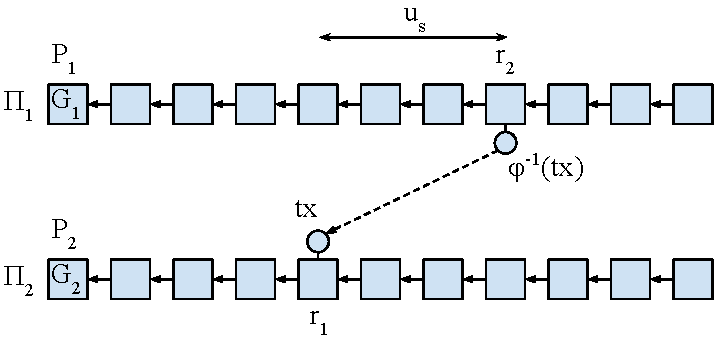
\includegraphics[width=0.8\columnwidth]{figures/bridge-safety.pdf}
    \caption{Bridge safety}
    \label{fig:bridge-safety}
\end{figure}

\paragraph{Bridge Liveness.}
Bridge liveness ensures that a transaction which appears on the source side will eventually make
it to the destination side. Intuitively, this guarantees that \emph{good things happen}, that is whenever an
honest party attempts to cross the bridge, it will successfully do so.
A visual depiction of bridge liveness is shown in Figure~\ref{fig:bridge-liveness}.
% Even though our treatment is general to all ledger protocols and not particular to blockchains,
% here we illustrate a blockchain example. 
A block containing transaction $\tx$ appears in the source side ($\Pi_1$) in the view
of a party $P_1$ at time $r_1$. Soon after, in round $r_2 \leq r_1 + u\ell$, the corresponding transaction image
$\phi(\tx)$ appears in the view of another party $P_2$ on the destination side ($\Pi_2$).

\begin{figure}
    \center
    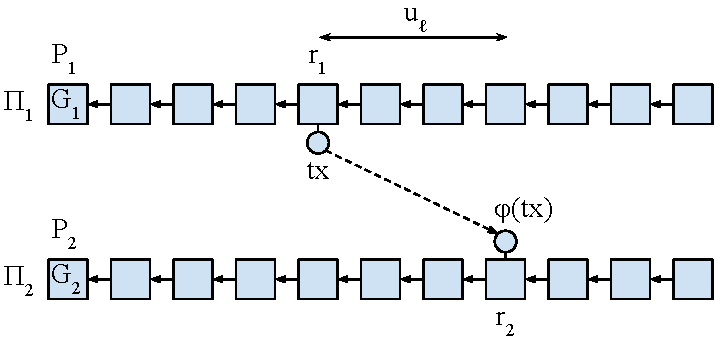
\includegraphics[width=0.7\columnwidth]{figures/bridge-liveness.pdf}
    \caption{Bridge liveness}
    \label{fig:bridge-liveness}
\end{figure}

\subsubsection{Light Clients}

A \emph{light client} is a client that wishes to synchronize with the rest
of the network, but has limited resources available in terms of communication,
computation, and storage. One example of a limited resource computer is the
on-chain smart contract infrastructure of Axelar, where computation and storage
are expensive. The light client begins its lifecycle holding the genesis block
and synchronizes to the current tip of the canonical chain once in a while.
Our job when building a light client is, given a block that the light client
has already downloaded sometime in the past, to allow the client to
synchronize with the most recent chain tip.

% TODO(shresth): Add a separate section before this to describe
% the high-level architecture of the on-chain light client without
% discussing the particularities of the Ethereum sync committee.
% Concretely, talk about how the data moves from Ethereum to
% Axelar when validators are dishonest and how they can be caught.

% TODO(shresth): Add a figure here.

\subsubsection{Ethereum Sync Committee}\label{subsec:sync-committee}

One useful ingredient of the Ethereum ecosystem that enables the
construction of efficient light clients is the so-called \emph{sync committee}~\cite{sync-committee}.
This feature was introduced in the system's
``Altair'' hard fork and is specifically tailored for use of light clients, as
we will discuss in the alternatives of Section~\ref{subsec:alternatives}.

The sync committee consists of $512$ of Ethereum validators. They are randomly
selected, from the set of all validators, every sync committee period (approx.
$1$ day).

Each honest validator in the sync committee is continually online and signs the
header of each block that is added to the chain's tip on every slot. The sync
committee is decided two periods before it takes effect. The root of the Merkle
tree that defines the committee is published in the header of a block in the
immediate period before the committee is activated. Consequently, when a block
is validated in this period, the committee is authorized to take effect (at the
beginning of its designated period).

We demonstrate the usage of the sync committee with the following example.

Assume that a client $C$ holds the block header of some slot $N$, that is part
of the sync committee period $X$.

When $C$ wants to authenticate the header of a block at slot $N'$, which is
part of the period $X+1$, it proceeds as follows.

First, $C$ validates the sync committee of period $X+1$. To do so, it verifies
that the Merkle root of the committee was published in a block header of period
$X$.

Following, $C$ updates its sync committee for $X+1$ as the one defined in the
Merkle tree. At this point, $C$ can validate every block header for each slot
of period $X+1$, by obtaining the corresponding signatures of the sync
committee of that period.

Using this iterative process, the light client can validate all future blocks,
starting from an initial trusted point. The cost of updating the sync committee
depends on the size of the committee, the aggregate signature, and the Merkle
path; in Ethereum this is estimated to approx. $25$KB~\cite{sync-committee}.

There are two main points of discussion around the sync committee.

First, the committee should be honest. In essence, the sampling process, via
which the sync committee's members are chosen from the set of all Ethereum
validators, should be secure, s.t. the probability that $\frac{2}{3}$ of the
committee members are adversarial is negligible. Observe that, if the committee
is malicious, then it can convince a light client of a fraudulent Ethereum
state. In a sense, this is a similar problem as the one identified in the
previous solution. Nonetheless, this problem has been extensively researched by
the Ethereum community, so the current election mechanism should be more secure
than any ad hoc solution that could be used in the first alternative above.

Second, there do exist incentives for participating honestly in the sync
committee~\cite{sync-committee-incentives}. In particular, a committee member
receives a reward for every slot during which it participates (that is sign a
block's header). A member also incurs a penalty for non participation (that is
either abstaining or signing the wrong header), equal to the reward it would
have received if participating.
However, slashed validators \emph{can} be selected as members of the sync
committee, for some period of time after the slashing occurs. This results in
complex dynamics, in terms of incentives, which is unclear whether they could
affect Axelar's implementation.
